\part{Framework}



\chapter{Overview}



一个好的库或者框架可以抽象一些复杂的开发工作,从而允许用户更快地编程,这样就可以极大地提高用户的生产力。


框架(framework)是一个基本概念上的结构,用于解决或者处理复杂的问题,框架的广泛定义经常被用于软件开发和机械结构和土木工程中。

土木工程中的框架是指由梁和柱等构件通过刚性连结组成的能承受垂直和水平荷载的结构体系,可以作为工业与民用建筑物的承重骨架、桥梁构架或工程构筑物等。

软件工程中的框架有不同的应用和意义,可以从不同的方面给出定义。

\begin{compactitem}
\item 从应用方面来定义框架,可以将其看作是整个或部分系统的可重用设计,表现为一组抽象构件及构件实例间交互的方法。
\item 从目的方面来定义框架,可以将其看作是可被应用开发者定制的应用骨架。
\end{compactitem}

从软件设计角度来看,框架是一个可复用的软件架构解决方案,其中规定了应用的体系结构,并且阐明了软件体系结构中的各个层次间及其层次内部各组件间的依赖关系、责任分配和控制流程,并最终表现为一组接口,抽象类以及实例间协作的方法。

通俗地说,框架就是某种应用的半成品,其本质是一组可以供用户选择来完成自己的系统的组件,因此可以认为是使用别人搭建好的舞台,自己来做表演。



作为可复用的设计构件,框架规定了应用的体系结构,阐明了整个设计、协作构件之间的依赖关系、责任分配和控制流程,并最终表现为一组抽象类以及其实例之间协作的方法。例如,Yaf框架中的Yaf控制器需要继承的类就是Yaf\_Controller\_Abstract。

\begin{lstlisting}[language=PHP]
<?php
class IndexController extends Yaf_Controller_Abstract{
	public function indexAction($name, $value){
	}
}
?>
\end{lstlisting}

构件复用提供了上下文(Context)关系,因此构件库的大规模重用也需要框架。另外,构件领域框架方法在很大程度上借鉴了硬件技术发展的成就,可以看作是构件技术、软件体系结构研究和应用软件开发三者发展结合的产物。


\section{History}

框架的概念最早起源于Smalltalk环境,其中最著名的框架是Smalltalk 80的用户界面框架MVC(Model-View-Controller)。

随着用户界面框架Interviews(Linton 89)和ET++(Weinand 89)的开发和发布,框架研究越来越受到研究人员的重视。虽然框架研究最初起源于用户界面领域,但是框架迅速被成功地应用到其他领域中,例如如操作系统(Russo 90)和火警系统(Molin 96a,Molin 96b)等。



现在的框架一般是成熟的,不断升级的软件,不过实际应用中的框架往往是不易变的,通常也不需要维护。只要基于框架开发的应用稳定运行,那么并不一定需要对框架进行不断升级。

框架可以看作是应用的底层架构(类似于C标准库),Ralph Johnson为框架所给出的定义基本上为大多数研究人员所接受:


\begin{compactitem}
\item 从框架内涵的角度可以将框架定义为一个可复用设计,由一组抽象类及其实例间协作关系来进行表达。

\item 从框架用途的角度可以将框架定义为在一个给定的问题领域内,一个应用程序的一部分设计与实现。
\end{compactitem}

从以上两个定义可以看出,框架是对特定应用领域中的应用系统的部分设计和实现,或者说半成品。

框架将应用系统划分为类和对象,定义类和对象的责任,类和对象如何互相协作,以及对象之间的控制线程,因此这些共有的设计因素由框架预先定义,应用开发人员只须关注特定的应用系统特有部分。

框架刻画了其应用领域所共有的设计决策,而且尽管框架中可能包含用某种程序设计语言实现的具体类,但是总的来说,框架着重于设计复用。

一个基于框架开发的应用系统可以包含一个或多个框架(例如Spring、Struts、Hibernate),与框架相关的构件类,以及与应用系统相关的功能扩展。

其中,与应用系统相关的扩展包括与应用系统相关的类和对象,实际的应用系统可能仅仅复用了面向对象框架的一部分,或者说,它可能需要对框架进行一些适应性修改来满足系统需求。

面向对象的框架作为一种可复用的软件,在基于框架的软件开发过程中会涉及到框架的开发和利用两个方面的工作。

框架的开发阶段在于实现领域中的可复用的设计,该阶段的主要结果是框架以及与框架相关的构件类,在后续的框架的的演变和维护中,还可能需要引入新的变化来应对错误处理和业务领域变化等。

不论是哪一种计算机技术,最终都是为业务发展而服务的。例如,从业务的角度来讲,框架首先需要为企业的业务发展和战略规划服务,服从于企业的愿景,而且框架最重要的目标是提高企业的竞争能力(包括降低成本、提高质量、改善客户满意程度以及控制进度等)。

框架实现其目标的方式是进行有效的知识积累,软件开发过程中的知识的聚集和积累是至关重要的,框架的作用就是采用一种结构化的方式对某个特定的业务领域进行描述,从而将这个领域相关的技术以代码、文档和模型等方式固化下来。


\section{Library}


虽然在很多情况下,框架通常以构件库的形式出现,不过用户需要明白的是构件库只是框架的一个重要部分,框架的关键在于框架内对象间的交互模式和控制流模式。

框架比构件(例如库)的可定制性强,因此在某种程度上,可以将构件和框架看成两个不同但彼此协作的技术。其中,框架为构件提供重用的环境,为构件处理错误、交换数据及激活操作提供了标准的方法。

应用框架并不是包含构建应用程序的片段程序,而是实现了某个应用领域的通用完备功能(除去特殊应用的部分)的底层服务,这样用户就可以在一个通用功能已经实现的基础上开始具体的系统开发。

框架提供了所有应用期望的默认行为的类集合,这样具体的应用就可以通过重写子类(该子类属于框架的默认行为)或组装对象来支持应用专有的行为。

应用框架强调的是软件的设计重用性和系统的可扩展性,以缩短大型应用软件系统的开发周期,提高开发质量。

与传统的基于类库的面向对象重用技术相比,应用框架更注重于面向专业领域的软件重用,而且应用框架具有领域相关性,用户可以根据框架对构件进行复合而实现可运行的系统。框架的粒度越大,其中包含的领域知识就更加完整。



\section{Feature}

软件开发(特别是服务器端软件)涉及到的知识、内容和问题太多,如果在某些方面使用成熟的框架,就相当于由别人完成基础工作,自己只需要集中精力完成系统的业务逻辑设计。

成熟、稳健的框架可以处理好系统的很多细节问题,比如事物处理、安全性、数据流控制等,另外框架一般都具有良好的结构和可扩展性,而且可以不断升级来直接获得框架升级带来的好处。

根据抽象层次,框架一般都是作为低层应用平台(如J2EE)和高层业务逻辑之间的中间层,这样就可以让软件系统具有“高内聚、低耦合”的特性,使得问题可以被划分开来各个解决,易于控制,易于延展。

除了框架和库的区别之外,框架和设计模式也有很大的不同。具体来说,构件通常是代码重用,设计模式则是设计重用,框架则介于两者之间,部分代码重用,部分设计重用,有时分析也可重用。

框架可以重用代码,可以很容易地从已有地构件库中建立自己地应用,构件一般都采用框架统一定义的接口,从而使构件间的通信简单。

框架可以重用设计,并且提供可重用的抽象算法及高层设计,这样就能将大系统分解成更小的构件,而且能描述构件间的内部接口。这些标准接口使在已有的构件基础上通过组装建立各种各样的系统成为可能。只要符合接口定义,新的构件就能插入框架中,构件设计者就能重用构架的设计。

框架可以重用分析,所有的人员若按照框架的思想来分析事务,那么就能将其划分为同样的构件,采用相似的解决方法,从而使采用同一框架的分析人员之间可以进行良好的沟通。

框架能提供的最大好处就是重用,面向对象系统获得的最大的复用方式就是框架,因此一个大的应用系统往往可能由多层互相协作的框架组成。

在软件生产中有三种级别的重用,分别是内部重用、代码重用和框架重用。

\begin{compactitem}
\item 内部重用就是在同一应用中能公共使用的抽象块;
\item 代码重用就是在多个应用和领域都能使用的通用模块组合成的库或工具集;
\item 应用框架的重用就是为专用领域提供的通用的或现成的基础结构,可以获得最高级别的重用性。
\end{compactitem}


框架与设计模式只是具有一定的相似性,但是二者之间有着根本的不同。

\begin{compactitem}
\item 框架可以用代码表示,也能直接执行或复用,而对模式而言只有实例才能用代码表示。
\item 设计模式比框架更抽象,只是对在某种环境中反复出现的问题以及解决该问题的方案的描述。
\end{compactitem}

设计模式是比框架更小的元素,一个框架中往往含有一个或多个设计模式,框架总是针对某一特定应用领域,但是同一模式却可以适用于各种应用,因此可以说,框架是软件,而设计模式是软件的知识。


\section{Prototype}

框架的优势在于快速原型技术,而且大粒度的重用进一步降低了开发费用,加快了应用逻辑的实现速度,降低了维护费用。

参数化框架增强了适应性和灵活性,在配置好框架后就可以可以直接重用代码,这样使得效率和质量都得到了提高。

框架使得用户专注于对领域的了解,需求分析更充分,而且软件结构一致性好,从而建立更加开放的系统。


框架要解决的最重要的一个问题是技术整合的问题,不同的软件企业可以根据应用自身的设计和具体的实现技术解耦,在J2EE框架中整合的各种各样的技术使得软件企业可以集中精力处理应用的设计,而不是具体的技术实现。

虽然最终的应用依赖于这些技术,但是应用底层的技术实现不应该对应用产生直接影响,否则技术自身的复杂性和技术的风险性将会直接对应用造成冲击。

例如,一个提供视频流应用并为电广行业提供整体的解决方案的软件企业的优势在于将各种各样的视频硬件、服务器、和管理结合起来,因此实际扮演的是一个集成商的角色,那么其核心价值在于使用软件技术将不同的硬件整合起来,并在硬件的整合层面上提供一个统一的管理平台,那么就应该放在解决下面两个问题。

首先,如何找到一种方法在思路上将不同的硬件整合起来,并且考虑的绝对不是要使用什么技术,而是这些硬件需要提供哪些服务,需要以什么样的方式进行管理,这样就可以在高层次上对领域进行建模。例如,可以定义任何一种硬件都需要提供两种能力,一种是统一的管理接口,用于对所有硬件统一管理;另一种是服务接口,系统平台可以查询硬件所能够提供的服务,并调用这些服务,设计的规范针对两种能力进行。

其次,如何描述这个管理系统的规范,例如各种管理活动,以及管理中所涉及的不同实体。管理系统实际上是针对硬件的管理,所以是构架在硬件整合平台之上的。

在完成业务层面的设计之后,再来看看具体的技术实现。只有规范和设计是不够的,还需要选择一个优秀的技术。例如,这里可以使用Java提供的JMX技术来对不同硬件进行整合。

根据JMX定义的通用规范以及远程管理端口的默认实现,可以在应用服务器中采用以JMX为基础的结构(例如JBoss),因此JMX为系统提供了一个很好的原型作为开始,接下来需要做的就是在JMX的基础上进行业务开发。

\section{Concepts}

框架可分为白盒(White-Box)与黑盒(Black-Box)两种,其中:

\begin{compactitem}
\item 基于继承的框架被称为白盒框架。
\item 基于对象构件组装的框架就是黑盒框架。
\end{compactitem}

\subsection{White-Box}


白盒具备可视性,被继承的父类的内部实现细节对子类而言都是可知的。

应用开发者基于白盒框架可以通过衍生子类或重写父类的成员方法来开发系统,因此子类的实现很大程度上依赖于父类的实现,这种依赖性限制了重用的灵活性和完全性。

为了解决白盒框架的局限性,可以只继承抽象父类,因为抽象类基本上不提供具体的实现,那么白盒框架就可以看作是一个程序骨架,用户衍生出的子类是这个骨架上的附属品。

\subsection{Black-Box}

应用开发者基于黑盒框架可以通过整理、组装对象来获得系统的实现。用户只须了解构件的外部接口,无须了解内部的具体实现,而且组装比继承更为灵活。

黑盒框架可以动态地改变,因此继承只是一个静态编译时的概念,这样在理想情况下,任何所需的功能都可通过组装已有的构件得到。

事实上,从黑盒框架可以获得的构件远远不能满足需求,有时通过继承获得新的构件比利用已有构件组装新构件更容易,因此白盒和黑盒将同时应用于系统的开发中。不过白盒框架趋向于向黑盒框架发展,黑盒框架也是系统开发希望达到的理想目标。

\subsection{Hot-spot}

成功的框架开发需要确定领域专用的“热点”(Hot spot),应用开发者在框架的基础上进行开发时只需要扩展框架的某些部分。

“热点”实际上就是在应用领域的一种扩展槽,开发者根据自己的需要填充这些扩展槽,因此“热点”就可以使框架具有灵活性。例如,在具体的实现中,扩展槽可以被看成是一些抽象类,开发者通过重写抽象方法获得具体实现。

\subsection{Cookbook}


“食谱”(Cookbook)是描述如何使用框架方法的文档,在“食谱”中包含了许多“烹饪”方法,这些“烹饪”方法相当于一些具体的操作步骤,描述了为解决某一专门问题如何使用框架的详细方法,不过框架的内部设计和实现细节通常不会出现在“食谱”中。

\subsection{Hollywood}

框架的一个重要特征就是用户定义的方法经常被框架自身调用,而不是从用户的应用代码中调用,这种机制经常被称为“好莱坞原则”(Hollywood Principle)或“别调用我们,我们会调用您”。


\begin{lstlisting}[language=PHP]

\end{lstlisting}

\section{Architecture}



随着管理信息应用范围的拓展,交易类应用为管理对象的电子信息获取提供了丰富的手段,这些信息的存储、加工、增值、展现等处理事务,均属于管理决策类应用系统的范畴。

传统的信息系统通常将这些事务,与交易类应用合并在一个应用系统中实现,随着一个组织中应用系统不断地涌现,关联数据的组织和共享、历史数据的积累和重用、全面数据的挖掘和增值等需求,促生了基于数据仓库技术的,面向整个组织,独立性的管理决策类应用环境的实现。

这类应用有一个最大的特点,就是用户需求是持续发展和不断完善的,特别是应用的初期,用户甚至提不出充分和全面的需求。同时,这类应用又存在非常强的应用共性。为此,可以通过一组与业务无关的,产品化的技术支撑环境,去实现对海量数据获取和储存的支持能力;去实现描述加工规则发展和完善的能力;去实现提供数据组织访问和管理的能力;去实现反映结果信息简洁和人性化的能力,这便是“管理决策框架”的意义。


\subsection{Business}


所有的应用系统只有在覆盖了相应的业务以后,才具有应用的实际意义。

与业务无关的管理决策框架在没有加载业务以前,只能称之为框架,加载业务以后则成为了针对特定业务的管理决策系统了。

所谓业务架构一方面是为用户加载和组织业务提供的一个手段和环境(开始也为用户加载了一些通用的业务如查询、报表等);另一方面也是在实际应用时的业务门户。

类似于智能终端的桌面,用户拿到手的时候桌面是空的,只是有一些通用业务,如时钟、画图、记事簿等,随着应用的发展,每个人的桌面会呈现出各不相同的个性化业务。管理决策框架中向用户提供了业务操作和管理的操作2类业务,其中业务操作是面向大众用户的,涉及业务管理活动的流程、查询、分析、决策等日常作业,这些操作绝大多数都需要用户后续自行加载;管理操作是面向小众用户的,涉及对业务管理活动的流程定义、数据组织、分析规则、决策算法、展现效果等定义和描述操作,并对它们进行加载和维护的作业。

与传统的应用系统不同的是,这些作业的形成不是由程序员编码实现的,而是用户骨干或者第三方团队(小众用户),利用管理决策框架提供的管理操作(由应用架构的相关产品提供)加载实现的。加载的结果通常以“方案”的形式打包,每个“方案”对应一个管理活动的过程、规则、算法、结果展现等等。训练成熟的方案经过该架构的解析和执行,面向用户提供直观高效的,可持续发展的,智能化的最佳用户体验。该架构涉及的技术包括:统一门户、统一权限、工作流、商务智能(BI)等等。



\subsection{Application}

应用架构主要是面向业务架构提供软件功能的支持,既提供运行时的业务功能支持,又提供加载时的管理功能支持。

与传统的应用架构的最大不同在于,该架构能为整个组织实现业务需求的变化和满足覆盖地域的不同,提供可持续发展的支撑能力和具有更长的生命周期。同时,也是确保业务无关性,实现管理决策类应用产品化的关键。为此,组成该架构的一系列产品,均以人机交互的模式,将管理决策业务需要实现的数据源获取、数据口径描述、数据的组织、加工规则、管理过程、结果展现等进行定义、描述和发布管理;其所涉及的每个定义和描述的结果,均分为2个部分,一是以代码段或脚本形式保存的,可以由业务架构解析并执行的部分,称为“方案元”;二是对相应的方案元按照标准的元模型,以人工语境描述的数据集合,称为“元数据”。方案元也作为元数据的一部分一并打包,并加以保存和管理,每项业务所涉及方案元的集合称为“方案”,每个“方案”经过测试和训练,面向特定的用户发布。这个过程称为“主动式元数据管理”。

应用架构发布的结果就是业务架构面向大众用户提供的“业务功能”;使用应用架构所提供产品进行业务实现(加载)的过程,就是小众用户在业务架构中使用“管理功能”的过程。该架构涉及的技术包括:元数据标准、元数据管理、方案的形成和管理、知识的形成和管理等等。


\subsection{Data}

数据架构面向全局提供统一的数据综合利用及管理环境。与传统的数据架构不同,该架构提出了对“数据空间 ”进行“数据管理”的概念。

“数据空间”是整个组织所有管理对象所涉及的数据全集,以及它们所有的数据属性。传统的数据架构关注的重点,局限在所有管理对象涉及的实体数据(内容),而“数据空间”关注和管理的对象,还要扩展到:一是以人工语境对“内容”进行解释性描述的元数据(变化);二是记录“内容”和“变化”的归档数据(历史);三是反映管理决策框架运行环境的日志数据(状态)等。这里记录内容、变化、历史、状态的数据集合,称之为“数据全集”;“变化”与传统的只供机器识别的技术元数据(传统数据属性),一并称之为新的“数据属性”。

“数据管理”指的是要对进入管理决策框架的数据源进行完整性、原始性、不可抵赖性的实现管理;要对基础数据口径和后续加工规则、算法等进行标准化、规范化、可追溯的描述管理;要对数据空间涉及的所有数据,进行合理组织、物理分区、数据结构的定义,实现全面科学、统分结合、访问高效的控制管理;要对内容、变化、历史、状态等涉及的所有数据增值过程,进行全面质量管理和全过程的生命周期管理。该架构涉及的技术包括:非结构化数据处理、档案管理、“大数据”技术、数据仓库(特别是DW2.0)涉及的相关技术等等。

\subsection{Technology}

技术架构是构成信息系统物理环境的产品集合,包括服务器、操作系统、中间件、网络环境等基础技术环境。在进行配置管理时,管理决策框架除了要考虑灾备的异地支持环境,还要在物理上分为生产环境和训练环境。生产环境是训练环境的子集,其主要是将正式发布的“方案”经过加载、解析、执行,针对特定业务提供日常作业的支持服务,从而确保了生产环境的简化、高效、可靠、稳定;训练环境除了能模拟实际生产环境,还要提供业务(方案)加载、测试、训练、维护、发布等管理作业的支持服务,从而确保该框架对业务应用无关性、对业务需求的可持续发展、保证支持环境的长生命周期。该架构涉及的技术包括:虚拟技术、云计算、容灾管理、数据中心监控等等。

\subsection{Security}

在最大限度满足管理决策框架运行的基础上,构建网络、硬件和软件相结合的安全体系,通过监控管理手段来确保系统稳定,削弱高度信息化的应用系统受单点故障的影响程度,使系统能够将风险分散和具备一定的自救能力。

要考虑一体化的,整体安全架构的设计要求;要符合信息安全标准(物理安全、运行安全、数据安全、内容安全等)规定而采取的技术和管理要求;要实现信息安全和数据质量管理的技术环境,能够提供安全策略的具体管理机制。信息安全不仅体现在物理环境的实现上,更要强调信息安全管理机制的建立和持续完善,并且管理机制要能够体现在物理环境上,要能够通过物理环境管理、记录、分析各类信息安全事件,避免其再次发生。


\subsection{Standard}

作为与业务无关的应用软件产品,管理决策框架需要一系列标准,以规范整个框架对外部的衔接、规范框架内各架构间的衔接,以及每个架构内部的,对处理对象的获取、加工、处理等描述的规范等等。

标准体系涉及到相互衔接、处理对象描述、加工规则描述等等方面的标准化,以及如何对它们进行描述的标准化(元数据标准,即元模型);涉及到包括组织、制定、维护、发布、遵循等内容的标准管理机制;特别是要有一个支撑标准管理机制的技术支持环境,这个环境不仅要提供对每个标准生命周期的管理,还要提供整个框架对标准遵循和使用的一致性和易用性保障和服务。


\subsection{Maintenance}



管理决策框架的运维体系分为2类:一类是物理环境运维。即传统的数据中心环境和设备的运行保障和安全保障;另一类是应用环境运维。它包括涉及业务架构、应用架构、数据架构、标准体系的运维管理。

通过这些运维管理活动,实现业务需求的有效支撑和可持续发展;实现管理功能(即整个框架本身)的可靠运行和可持续发展。为了这2类管理活动的有效进行,需要建立一套运维管理机制,包括运维组织、制度、职责等等;同样,也要有一个支撑运维管理活动的运维技术支持环境,它不仅要提供对运维管理活动的过程和监控提供服务,还要提供对运维事项的发起、发现、定位、预警、处置、恢复等手段提供功能性支持,并且能够通过对运维事件多角度信息的捕获、积累、分析、挖掘,实现智能化的运维辅助和事件预测。


\begin{lstlisting}[language=PHP]

\end{lstlisting}


\section{Software Framework}

软件框架(Software framework)通常指的是为了实现某个业界标准或完成特定基本任务的软件组件规范,也指为了实现某个软件组件规范时,提供规范所要求之基础功能的软件产品。

框架的功能类似于基础设施,与具体的软件应用无关,但是提供并实现最为基础的软件架构和体系。软件开发者通常依据特定的框架实现更为复杂的商业运用和业务逻辑,这样的软件应用可以在支持同一种框架的软件系统中运行。

简而言之,框架就是制定一套规范或者规则(思想),用户可以在该规范或者规则(思想)下工作,或者说使用别人搭好的舞台来做编剧和表演。

\section{Web Framework}


\subsection{Overview}


Web application framework(Web应用框架)可以用来支持动态网站、网络应用程序及网络服务的开发,这样就可以减轻网页开发时共通性活动的工作负荷。例如,许多Web应用框架往往提供了数据库访问接口、标准模板以及会话管理等,从而提升代码的可复用性。

许多Web应用框架遵循模型 - 视图 - 控制器(MVC)体系模型的结构模式,使数据模型与用户界面分开,并且通过模块化的代码提高代码的重复使用,同时允许多个接口。

Web应用程序通常可以划分为客户端、应用程序和数据库三个部分,其中数据库通常是一个RDBMS,客户端是由Web应用程序生成的HTML,并且在用户的浏览器运行,应用程序在服务器上运行。

\subsection{Web Template}



\begin{lstlisting}[language=PHP]

\end{lstlisting}


\subsection{Web Caching}







\begin{lstlisting}[language=PHP]

\end{lstlisting}



\subsection{Web Security}





\begin{lstlisting}[language=PHP]

\end{lstlisting}



\subsection{Data Mapping}


\begin{lstlisting}[language=PHP]

\end{lstlisting}



\subsection{URL Mapping}


\begin{lstlisting}[language=PHP]

\end{lstlisting}


\subsection{Ajax Service}


AJAX(Asynchronous JavaScript and XML,异步的JavaScript与XML技术)是一套综合了多项技术的浏览器端网页开发技术。

传统的Web应用允许用户端填写表单(form),当提交表单时就向Web服务器发送一个请求。服务器接收并处理传来的表单,然后送回一个新的网页,但这个做法浪费了许多带宽,因为在前后两个页面中的大部分HTML码往往是相同的。由于每次应用的沟通都需要向服务器发送请求,应用的回应时间依赖于服务器的回应时间。这导致了用户界面的回应比本机应用慢得多。

与此不同,AJAX应用可以仅向服务器发送并取回必须的数据,并在客户端采用JavaScript处理来自服务器的回应。因为在服务器和浏览器之间交换的数据大量减少(大约只有原来的5\%),服务器回应更快了。同时,很多的处理工作可以在发出请求的客户端机器上完成,因此Web服务器的负荷也减少了。

类似于DHTML或LAMP,AJAX不是指一种单一的技术,而是有机地利用了一系列相关的技术。虽然其名称包含XML,但实际上数据格式可以由JSON代替,进一步减少数据量,形成所谓的AJAJ。

客户端与服务器也并不需要异步。一些基于AJAX的“派生/合成”式(derivative/composite)的技术也正在出现,如AFLAX。


\subsection{WebService}

\chapter{JavaScript}

框架(例如AngularJS、Backbone和Ember)可以将应用逻辑从服务端转移到前端,这样应用原来所需要的计算资源可以前移到客户的浏览器端,而且将应用的代码带入前端模糊了传统的前后端开发,这样就可以达到减少服务器压力和支出的效果。


\section{AngularJS}





\section{Backbone}





\section{Ember}





\chapter{Java}





\section{Struts}





\section{Spring}

Spring本身是开源而免费的,Tomcat是Spring应用程序最主流的运行平台





\section{Hibernate}



\chapter{PHP}


PHP的发展促使PHP框架层出不穷, 但是到底用不用PHP框架还存在很大的争论,反对者认为使用框架(例如Zend Framework)会降低性能,支持者则认为采用框架能提高开发效率,性能损失也是值得的。

在实际情况中,用户往往为了性能而选择某些框架,或者为了更好的封装来选择其他的框架,难以兼顾性能和开发效率。



\section{Yaf}


\subsection{Overview}


The Yet Another Framework(Yaf)扩展是一个用来开发Web应用的PHP框架,需要5.2.1及以上版本PHP,早期版本可能不能正常工作。

\begin{compactitem}
\item Yaf需要SPL的支持. SPL在PHP5中是默认启用的扩展模块
\item Yaf需要PCRE的支持. PCRE在PHP5中是默认启用的扩展模块
\end{compactitem}

yaf提供了和Zend Framework相似的API以及相似的理念,同时又保持着对Bingo的兼容,并以此来提高开发效率,规范开发习惯。

具体来说,yaf把框架中不易变的部分抽象出来,并使用C语言实现为PHP扩展来保证性能,可以做到比原生PHP小于10\%的性能损失,同时相比Zend Framework则产生50-60倍的性能提升。不过,框架的时间和真正应用逻辑的耗时相比只是很小的一部分。


测试用原生的PHP:orig.php

\begin{lstlisting}[language=PHP]
<?php
class IndexController{
	public function actionIndex(){
		echo "Laruence";
	}
}
$controller = new IndexController();
$controller->actionIndex();
?>
\end{lstlisting}

测试用的Yaf的入口文件:ap.php

\begin{lstlisting}[language=PHP]
<?php
$conf = array(
	"application.directory"=>"/home/laruence/local/www/htdocs/ap",
);

$app = new Yaf_Application($conf);
$app->run();
?>
\end{lstlisting}

测试用的Yaf的默认控制器:Index.php

\begin{lstlisting}[language=PHP]
<?php
class IndexController extends Yaf_Controller{
	public function actionIndex(){
		$this->disableView(); // 关闭视图输出
		echo "Laruence";
	}
}
?>
\end{lstlisting}

下面采用ab作为测试工具,并且分别在并发1, 100, 200的情况下对二者进行测试。

\begin{compactitem}
\item 1并发,请求1000次, 原生的PHP/Yaf

\begin{lstlisting}[language=PHP]
$ ./ab -n1000 -c1 http://127.0.0.1/orig.php

Document Path:          orig.php
Document Length:        8 bytes

Concurrency Level:      1
Time taken for tests:   0.463 seconds
Complete requests:      1000
Failed requests:        0
Write errors:           0
Total transferred:      130000 bytes
HTML transferred:       8000 bytes
Requests per second:    2159.41 [#/sec] (mean)
Time per request:       0.463 [ms] (mean)
Time per request:       0.463 [ms] (mean, across all concurrent requests)
Transfer rate:          274.14 [Kbytes/sec] received

Connection Times (ms)
              min  mean[+/-sd] median   max
Connect:        0    0   0.0      0       0
Processing:     0    0   0.2      0       5
Waiting:        0    0   0.2      0       5
Total:          0    0   0.2      0       5

Percentage of the requests served within a certain time (ms)
  50%      0
  66%      0
  75%      0
  80%      0
  90%      0
  95%      0
  98%      0
  99%      1
 100%      5 (longest request)
$ ./ab -n1000 -c1 http://127.0.0.1/ap/index.php

Document Path:          /ap/index.php
Document Length:        8 bytes

Concurrency Level:      1
Time taken for tests:   0.525 seconds
Complete requests:      1000
Failed requests:        0
Write errors:           0
Total transferred:      130000 bytes
HTML transferred:       8000 bytes
Requests per second:    1906.24 [#/sec] (mean)
Time per request:       0.525 [ms] (mean)
Time per request:       0.525 [ms] (mean, across all concurrent requests)
Transfer rate:          242.00 [Kbytes/sec] received

Connection Times (ms)
              min  mean[+/-sd] median   max
Connect:        0    0   0.0      0       0
Processing:     0    0   0.3      0       7
Waiting:        0    0   0.3      0       7
Total:          0    0   0.3      1       7
ERROR: The median and mean for the total time are more than twice the standard
       deviation apart. These results are NOT reliable.

Percentage of the requests served within a certain time (ms)
  50%      1
  66%      1
  75%      1
  80%      1
  90%      1
  95%      1
  98%      1
  99%      1
 100%      7 (longest request)
\end{lstlisting}

\item 100并发,请求1000次, 原生的PHP/Yaf

\begin{lstlisting}[language=PHP]
$ ./ab -n1000 -c100 http://127.0.0.1/orig.php

Document Path:          orig.php
Document Length:        8 bytes

Concurrency Level:      100
Time taken for tests:   0.287 seconds
Complete requests:      1000
Failed requests:        0
Write errors:           0
Total transferred:      130000 bytes
HTML transferred:       8000 bytes
Requests per second:    3478.82 [#/sec] (mean)
Time per request:       28.745 [ms] (mean)
Time per request:       0.287 [ms] (mean, across all concurrent requests)
Transfer rate:          441.65 [Kbytes/sec] received

Connection Times (ms)
              min  mean[+/-sd] median   max
Connect:        0    0   1.0      0       6
Processing:     5   27   4.8     27      35
Waiting:        5   27   4.8     27      35
Total:          6   27   4.6     27      36

Percentage of the requests served within a certain time (ms)
  50%     27
  66%     28
  75%     29
  80%     31
  90%     35
  95%     35
  98%     35
  99%     35
 100%     36 (longest request)
$ ./ab -n1000 -c100 http://127.0.0.1/ap/index.php

Document Path:          /ap/index.php
Document Length:        8 bytes

Concurrency Level:      100
Time taken for tests:   0.316 seconds
Complete requests:      1000
Failed requests:        0
Write errors:           0
Total transferred:      130000 bytes
HTML transferred:       8000 bytes
Requests per second:    3165.24 [#/sec] (mean)
Time per request:       31.593 [ms] (mean)
Time per request:       0.316 [ms] (mean, across all concurrent requests)
Transfer rate:          401.84 [Kbytes/sec] received

Connection Times (ms)
              min  mean[+/-sd] median   max
Connect:        0    0   1.0      0       6
Processing:     6   30   5.6     27      44
Waiting:        6   30   5.6     27      44
Total:          6   30   5.6     27      44

Percentage of the requests served within a certain time (ms)
  50%     27
  66%     32
  75%     34
  80%     36
  90%     37
  95%     40
  98%     42
  99%     42
 100%     44 (longest request)
\end{lstlisting}


\end{compactitem}

考虑到Yaf有1次IO操作(载入Controller),但是原生的PHP并没有, 那么基本可以认为使用了Yaf框架以后, 性能损失在2\%-10\%。




\begin{lstlisting}[language=PHP]

\end{lstlisting}



\begin{lstlisting}[language=PHP]

\end{lstlisting}



\begin{lstlisting}[language=PHP]

\end{lstlisting}



\begin{lstlisting}[language=PHP]

\end{lstlisting}





yaf并不是万能的,它只是解决了应用中的最基本的一个问题——就是框架带来的额外的性能开销,不过这部分的开销和应用实际的开销相比,往往是很小的。

在PHP已经提供了对DB的一个轻度封装的PDO的前提下,直接使用PDO比复杂的ORM包装会更加简单和高效,因此最初Yaf并不包含ORM。

在后续的Yaf的版本中会考虑加入ORM, 不过只是一个简单的ORM, 类似于Yaf的内建视图引擎(Yaf\_View\_Simple)。



如果需要在Ubuntu上安装yaf,可以执行下面的命令:


\begin{lstlisting}[language=PHP]
$ sudo add-apt-repository ppa:mikespook/php5-yaf
$ sudo apt-get update
$ sudo apt-get install php5-yaf
\end{lstlisting}

yaf框架本身被设计为一个PHP扩展,因此可以使用PECL来进行安装,不过大部分的主机提供商往往不允许用户自己安装PHP扩展,因此限制了yaf的应用。

\begin{lstlisting}[language=PHP]
$ sudo pecl install yaf
\end{lstlisting}




\subsection{Directory}


一个典型的应用目录结构如下:

\begin{lstlisting}[language=PHP]
- index.php 
- .htaccess 
+ conf
    |- application.ini  //application config
- application/
    - Bootstrap.php   
    + controllers
        - Index.php  //default controller
    + views    
        |+ index   
             - index.phtml  //view template for default action
    + modules 
    - library
    - models  
    - plugins 
\end{lstlisting}

其中,顶层目录下的index.php是整个应用的唯一入口,应该把所有请求都重定向到这个文件。




\begin{lstlisting}[language=PHP]
<?php
define("APPLICATION_PATH",  dirname(__FILE__));

$app  = new Yaf_Application(APPLICATION_PATH . "/conf/application.ini");
$app->bootstrap() //call bootstrap methods defined in Bootstrap.php
 ->run();
?>
\end{lstlisting}





在Apache+php\_mod模式下可以使用.htaccess来实现重写规则:

\begin{lstlisting}[language=PHP]
#for apache (.htaccess)
RewriteEngine On
RewriteCond %{REQUEST_FILENAME} !-f
RewriteRule .* index.php

#for nginx
server {
  listen ****;
  server_name  domain.com;
  root   document_root;
  index  index.php index.html index.htm;

  if (!-e $request_filename) {
    rewrite ^/(.*)  /index.php/$1 last;
  }
}

#for lighttpd
$HTTP["host"] =~ "(www.)?domain.com$" {
  url.rewrite = (
     "^/(.+)/?$"  => "/index.php/$1",
  )
}
\end{lstlisting}




\begin{lstlisting}[language=PHP]

\end{lstlisting}





\subsection{Compile}

虽然yaf使用C语言开发,但是无需编译,而且比原生的PHP几乎不会带来额外的性能开销。

yaf是一个全功能的PHP框架,而且比一般的PHP框架更快、更轻便,而且提供了Bootstrap、路由、分发、视图和插件等功能。

yaf提供的所有的框架类都不需要编译,在PHP启动的时候加载并且常驻内存。

yaf提供了更短的内存周转周期,提高内存利用率,降低内存占用率。

yaf的自动加载机制支持全局和局部两种加载规则,方便类库共享。


\begin{lstlisting}[language=PHP]

\end{lstlisting}


\subsection{Engine}

yaf作为高度灵活可扩展的框架,支持自定义视图引擎、插件和自定义路由等。

yaf内建多种路由,并且可以兼容常见的各种路由协议。

yaf提供了强大而又高度灵活的配置文件支持,并支持缓存配置文件,从而可以避免复杂的配置结构带来的性能损失。

在yaf框架本身,对危险的操作习惯进行禁止。

\subsection{Plugin}

虽然可以通过阅读框架代码并在框架代码中输出信息来进行调试,不过yaf本身提供了件机制来提供丰富的debug信息,并且专门为命令行下的调试做了特别优化,尽可能的在出现错误的时候,给予更多的错误原因。


\subsection{Kernel}

yaf的实现基于PHP的内核API,因此yaf的执行层面和PHP代码的执行层面相同,并且充分的注意了避免对PHP带来侵入性。



\subsection{Bootstrap}

Yaf提供了完善的API,并支持Bootstrap和插件机制,其整体流程图如下:

\begin{figure}[htbp]
\centering
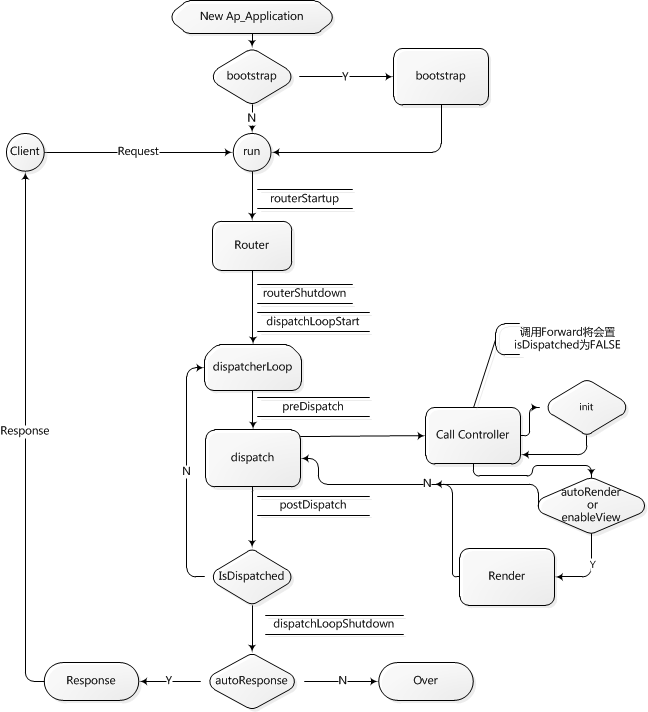
\includegraphics[scale=0.5]{yaf_sequence.png}
\caption{yaf的整体流程}
\end{figure}



\begin{lstlisting}[language=PHP]

\end{lstlisting}




\begin{lstlisting}[language=PHP]
<?php
define("APPLICATION_PATH",  dirname(__FILE__));
define("PUB_TPL",dirname(__FILE__)."/application/views");
require_once(APPLICATION_PATH."/Macro.php");
try {
	$app  = new Yaf_Application(APPLICATION_PATH."/conf/5bb88e1e53666ec494f1025023c16dea.ini");
	$app->bootstrap() //call bootstrap methods defined in Bootstrap.php
    ->run();
} catch (Yaf_Exception_StartupError $e) {

}

\end{lstlisting}




\begin{lstlisting}[language=PHP]

\end{lstlisting}



\begin{lstlisting}[language=PHP]

\end{lstlisting}




\begin{lstlisting}[language=PHP]

\end{lstlisting}




\begin{lstlisting}[language=PHP]

\end{lstlisting}




\begin{lstlisting}[language=PHP]

\end{lstlisting}




\begin{lstlisting}[language=PHP]

\end{lstlisting}







